\chapter{Pipeline}

\label{kap:pipeline} % id kapitoly pre prikaz ref
\paragraph*{}
Our pipeline uses a combination of various tools to modify input from Illumina sequenced paired-end reads. In this chapter, we explain used tools and their integration into the pipeline. 
\section{Seqtk}
\paragraph*{}
Seqtk\cite{li2012seqtk} is a tool capable of fast processing of sequences in FASTA or FASTQ format. In our pipeline, we use the ability of seqtk to extract a subsample of reads from an input file. By using the same random seed for two paired FASTQ files, we get a fixed set of paired reads with the requested number of sequences. The subsampling is especially useful when working with large files because due to the nature of SPAdes, which requires notably larger available memory than the size of the input files. If the client does not possess the required amount of memory, by using random subsampling, the tool is still able to assemble the sample into contigs. 

Lowering the number of reads results in shorter runtime of SPAdes at the cost of accuracy. At this stage our tool focuses on accuracy, so the number is set to the highest value. The value is adjustable for added flexibility allowing our tool to operate with lower memory demands.

\section{SPAdes}
\paragraph*{}
SPAdes\cite{bankevich2012spades} si a short read assembler designed for the assembly of small single-cell and multi-cell bacterial reads. While assemblies of viral DNA are not its speciality, it has been proven that SPAdes produces consistently accurate results even when compared to virus-oriented assemblers \cite{sutton2019choice}. SPAdes works on reads from Illumina and IonTorrent. It can also create hybrid assemblies using PacBio, Oxford Nanopore and Sanger reads. The reads from Illumina can be either paired-end, mate-pairs or single reads. The method used for assembly is based on using k-mers, subsequences with a length of k from reads, to create a de Bruijn graph on which further theoretical operations are executed. The assembler also performs an error adjustment, increasing the reliability of produced contigs.
\subsection{Terminology}
\paragraph*{}
To understand the algorithm SPAdes uses, several terms need to be explained. Hub is a vertice of a directed graph with the number of edges leading to it is different from one. The number of edges leaving it is different from one as well. When two hubs are connected by a path of non-hub vertices, the path is called a hub-path (h-path). Each edge in the graph belongs to a unique h-path. For every h-path, its first edge is called a hub-edge (h-edge).

\subsection{Algorithm}
\paragraph*{}
The algorithm of SPAdes can be simplified into four stages: assembly graph construction, k-bimer adjustment, paired assembly graph construction and contig construction \cite{bankevich2012spades}. 

The first stage begins with the construction of a multisized de Bruijn graph. This graph is created from k-mers by creating vertices with the first labelled by the prefix of the k-mer and the second by its suffix. These vertices are connected by an edge representing the k-mer. Merging vertices with the same labels results in the creation of a de Bruijn graph. To make this graph multisized, a different value of k is used based on the coverage of a region. In regions with lower coverage, the value of k used is lower. Conversely, in high-coverage regions, the value used is higher. 

With the graph created, SPAdes locates and corrects errors in the graph caused by errors in reads. To discover which h-paths in the graph are correct, it implements an improved gradual h-path removal strategy. One of the improvements lies in iterating through h-paths and updating the list of h-paths as soon as one is removed. It also at some points runs only bulge corremovals, which are considered safer than other removals, because they maintain information on removed h-paths. Lastly, it restricts the removal of h-paths to only those, which start with a hub with at least two outgoing edges and end with a hub with at least two incoming edges. For tips, this restriction only applies to the hub which has both incoming and outgoing edges. Every type of error corrected using this strategy has a procedure designed to fix it \cite{bankevich2012spades}.

\begin{figure}[h]
  \begin{center}
     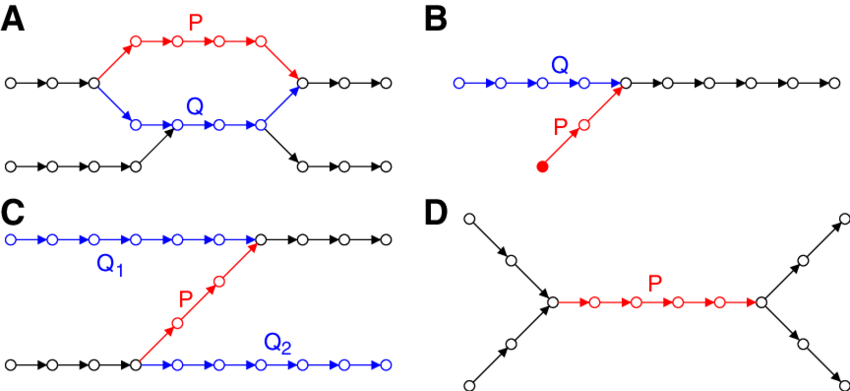
\includegraphics[width=0.5\textwidth]{images/errors.png}
     \caption{Potential errors in the graph: bulge (A), tip (B), chimeric read (C), repeat (D) \cite{bankevich2012spades}.}\label{fig:errors}
  \end{center}
\end{figure} 

Miscalled bases and indels in the read tend to create two distinct paths, with at least one being an h-path, connected to the same start and stop hubs, called bulges (Figure \ref{fig:errors}A). To fix these bulges, SPAdes uses a procedure called "bulge correction and removal" (bulge corremoval). In this method, SPAdes iterates through all h-paths in increasing order of coverage. Once it locates a bulge, from the two paths forming the bulge, every edge of the h-path is mapped to an edge in the other path. After the mapping, the mapped path is removed from the graph, and the coverage of the remaining path is increased. The information about the path removed in the corremoval is stored in a map, which makes it possible to backtrack corremovals. SPAdes takes advantage of the backtracking of corremovals later when creating a paired assembly graph.

Errors at the start or end of a read can lead to a sequence of multiple stray edges protruding from the graph called tip (Figure \ref{fig:errors}B). SPAdes determines, whether an h-path is a tip by considering whether there is an alternative h-path, if the length of the h-path is below a specified threshold and if the average coverage of the h-path is below a specified threshold. To perform the removal of tips, SPAdes iterates through all h-paths in order of ascending length up to the length threshold. Each h-path satisfying the conditions of being a tip is removed from the graph. When a path is removed, the parameters of the affected part of the graph are recomputed to reflect the new version of the graph. This makes it possible to remove all tips in a single iteration through the graph.

Chimeric reads and incidental short overlaps between reads sometimes lead to the creation of chimeric h-paths (Figure \ref{fig:errors}C). For an h-path to be considered chimeric, its start hub has to have at least two outgoing edges and its stop hub has to have no more than two incoming edges, and its length and coverage must be below a specified threshold. Additionally, some heuristics are employed to remove chimeric h-paths that do not satisfy the coverage limit because of amplification in the reads. To find h-paths satisfying the conditions, SPAdes iterates through all h-paths in order of ascending coverage.

After these graph simplifications, all isolated h-paths with lengths lower than 200 are removed.

In the second stage, SPAdes uses read-pairs to estimate the genomic distance between h-paths linked by them. The pair of h-paths is then connected by aggregation of the estimated distances between reads in read-pairs linking the h-paths. To connect the paths, read-pairs undergo a series of transformations \cite{bankevich2012spades}. 

In B-transformation, the read-pairs are transformed into k-bimers. Each k-bimer contains two k-mers from the read-pairs and a distance between the k-mers calculated as:
\[d - i_{1} + i_{2}\]
where $i_{1}$ and $i_{2}$ are starting positions of the k-mers on the reads and $d$ is the approximate genomic distance between reads. Since each k-mer is represented in the graph as an edge, the k-bimer is also referred to as a "biedge".

Following B-transformation, H-transformation transforms biedges into h-biedges. Every biedge defined by edges residing on h-paths undergoes this transformation. Since, as mentioned earlier, every edge in the graph belongs to an h-path, H-transformation is performed on all biedges. For biedge with edges $a$ and $b$ and distance between them $d$, an h-biedge $H(a|b,d)$ is constructed as follows:
\[ H(a|b,d) = (h-edge(a)|h-edge(b),D) \]
The variables $h-edge(a)$ and $h-edge(b)$ represent h-edge on the same h-path as the edge in question. The value of D is calculated as:
\[D = d + i_{a} - i_{b}\]
with $i_{a}$ ($i_{b}$) being an index of which edge from the beginning is $a$ ($b$). By executing this transformation, information about every h-biedge is collected into a histogram. Every histogram is a multiset of h-biedges with the same h-edges. Since the index for edges on the same h-path can be different, the distance estimate specified in h-biedge may vary.

After creating the h-biedge histogram, it undergoes A transformation. The histograms and the paths of the graph are analyzed by a fast fourier transform algorithm. The analysis derives accurate distance estimates between h-edges. Using an adjustment operation, each histogram is transformed into a small number of adjusted h-biedges with distance estimates.

The h-biedges adjusted with A-transformation are then used by E-transformation to recalculate distances between biedges. For each h-biedge $(\alpha|\beta,D)$, E-transformation creates a set of biedges $(a|b,d)$, where $a$ ($b$) belongs to the same h-path as $\alpha$ ($\beta$). Distance $d$ for each biedge is calulated in the same way as in H-transformation:
\[ d = D - i_{a} + i_{b} \]
where $i_{a}$ ($i_{b}$) is an index of which edge from the beginning is $a$ ($b$). The result of the transformation is a set of biedges with accurate distance estimates.

In stage three, SPAdes constructs a paired assembly graph. To construct a paired assembly graph, SPAdes attempts to find an Eulerian cycle consistent with all biedges in the de Bruijn graph \cite{bankevich2012spades}. An Eulerian cycle is considered consistent with a biedge if it contains instances of both edges from biedge at a distance specified in biedge. By creating a de Bruijn graph from a set of biedges where vertices are labelled as the start or stop of a biedge and directed edges labelled as biedges, the h-paths of the resulting graph are shared by the Eulerian cycles consistent with biedges. To reduce the time and memory requirements, SPAdes uses h-biedges to create the graph \cite{bankevich2012spades}. It creates a graph in a way, where vertices are labelled as start with the biedge with the lowest offset and stop with the biedge with the highest offset. The edge between the vertices is then labelled with the h-biedge. Since doing this only simplifies the graph, the h-paths in it are shared by Eulerian cycles consistent with biedges as well. The cycles are found in the assembly graph by pairing it with the h-biedge graph.

In the final stage, SPAdes outputs created contigs from the paired assembly graph. The contigs are represented by the h-paths in the paired assembly graph.

Since our tool is designed to work with paired-end reads, we use SPAdes in a configuration using the paired-ends library. Our tool also uses the default values for k-mers of 21, 33 and 55. Even though the input reads contain metagenomic data, we do not use metaSPAdes because we are unsure if technical sequences are present in the data and quality control could increase the runtime of the tool. For the same reason, we also avoid using -careful flag.

\section{Phanotate}
\paragraph*{}
Phanotate\cite{mcnair2019phanotate} is a gene caller designed to identify the location of genes in phage genomes. The location of a gene in the DNA is called an open reading frame (ORF). The DNA covered by an ORF is transcribed and further utilized. Phanotate identifies the location of genes by locating ORFs. Since gene callers designed to work specifically with phage genomes are sparse, the prediction of phage genes is more accurate compared to many different gene callers. It accomplishes this by working under two assumptions. Firstly, since the phage genome is limited by physical constraints, the genome needs to be compact \cite{kang2017prophage}. The compactness is partially provided by allowing a minimal amount of non-coding DNA. Secondly, because phage genes tend to be co-transcribed, they are ordinarily situated on the same strand of DNA \cite{akhter2012phispy}. Taking this into account, Phanotate handles the genome as a network of paths where ORFs are more favourable while overlapping ORFs and switching of DNA strains are less favourable. Phanotate then utilizes the Bellman-Ford algorithm to find the best path in the resulting weighted graph.

\subsection{Algorithm}
\paragraph*{}
First, Phanotate creates a weighted graph representing ORFs. As a start for ORF, it allows ATG, GTG and TTG codons. To end an ORF, codons allowed are TAA, TAG and TGA. By default, the minimal length of an ORF is set to 90 nucleotides. In the graph, the nodes represent only start and stop codons. Edges between them have different meanings depending on what nodes they connect. Edges connecting the start node with the following stop node in the same read frame and on the same strand of DNA represent ORF. Gaps are represented by edges connecting the stop codon and either subsequent start codon in any reading frame on the same strand or subsequent stop codon on an alternate DNA strand. Overlaps are also represented by edges connecting the stop codon. However, they connect to either the preceding start codon in another reading frame on the same strand or the preceding stop codon on an alternate strand. Since phages seldom have gaps between ORFs, only ORFs separated by around 300 bp and less are connected by an edge. If the sequence contains a large section of DNA without an ORF, the ORFs on both sides of the section are connected with an edge with a linear penalty.

The weight of the edges is calculated based on their nature. For the edge representing ORF, Phanotate calculates weight as an adjusted likelihood of not finding a stop codon in an ORF of the length. This is done by first counting the fraction of each base in each ORF. This then determines the probability of encountering a specific end codon, which is used to calculate the probability of encountering any stop codon:
\[ P(stop) = P(TAA) + P(TAG) + P(TGA) \]
Calculated probability is then used to calculate the probability of not encountering any stop codon:
\[ P(not stop) = 1 - P(stop) \]
The P(not stop) value is sufficient in genomes having an average content of nucleotides G and C (GC content). To avoid the creation of spurious ORFs with substantial length in genomes with high GC content, Phanotate utilizes minimum and maximum GC frame plots (GCFP). The GCFP are generated in several steps. 

First, three read frames of the genome are read starting from an appropriate base and looking at a codon starting with that base to calculate the percentage of GC bases on a 120 bp window of each frame. Next, by iterating through codons of a set of ORFs starting with the ATG codon, Phanotate determines, which position of codon has the highest GC content and maintains a running total for that position. For a minimal GC frame plot, the process determines the lowest GC content. This results in a set of frequencies of GC bases for each of the three positions in ORFs starting with the ATG codon. The frequencies are then used to estimate the favoured reading frame at any location. Each of the frequencies is then divided by the highest, resulting in values ranging between zero and one, with one being the maximal or minimal GC frame. These values are then used to exponentiate P(not stop).

The scores of ORFs are further modified by the weighted ribosomal-binding site (RBS) score. The RBS score is determined using the Shine-Dalgarno RBS system \cite{hyatt2010prodigal}. ORF scores are adjusted more by the probability of the first codon being a start. The probability is calculated as a normalized frequency of start codons from genes on 2133 phage genomes contained in GenBank. The weight of edges representing ORF is negated in the final calculation to denote them as favourable in the graph. The final calculation of the weight of the edge representing ORF is:
\[ w_{orf} = - \frac{1}{\prod\limits_{c=1}^{codons}(P(not stop)^{GCFPmax_{maxGCframe(c)} GCFPmin_{minGCframe(c)}})} * RBS * START \]

In cases, where the edge represents a gap or an overlap, the next ORF can be on any strand of the DNA. Since the phage genes tend to be on the same strand, the switch of strands is penalised by adding a multiplicative inverse of the probability of switch to the resulting weight of the edge. The probability is expressed by a variable P(switch) attaining a value of 0 or 0.05 calculated from a set of annotated genes from 2133 phage genomes available on GenBank.

The weight of the gap is calculated using a similar method to the weight of ORF. The differences are that gaps are not corrected by the GC frame plot and that the average probability of not finding a stop codon is genome-wide and exponentiated by the length of the gap. In the case of a switch, a multiplicative inverse of variable P(switch) is added to the multiplicative inverse of the calculated probability resulting in the equation:
\[w_{gap} = \frac{1}{\underline{P}(not stop)^{len}} + \frac{1}{P(switch)}\]

For edges representing overlaps, the weight is calculated as the average of the two weights of the ORFs in the overlap by the length of the overlap. Similarly to the weight of the gap, in the case of a switch, a multiplicative inverse of variable P(switch) is added, resulting in an equation:
\[w_{gap} = \frac{1}{(\frac{P(not stop)_{1} + P(not stop)_{2}}{2})^{len}} + \frac{1}{P(switch)}\]

The calculated weights are afterwards transformed into distances by using the multiplicative inverse. With the distances and nodes, the resulting weighted graph is processed by the Bellman-Ford algorithm. Phanotate then writes ORFs from the shortest path calculated by the algorithm as an output.

Our tool slightly modifies Phanotate. The reason behind this is that since Phanotate is designed to work on whole genomes, it assumes that every input sequence contains at least one ORF. However, our tool does not produce entire genomes for Phanotate to work on due to redundancy and a possible decrease in processing speed. Therefore, we modified the script so that if a sequence does not contain any ORFs, Phanotate will skip that sequence. We also set the format of the output as tabular, since when Phanotate exports output in fasta format, it does not include the information on which strand was an ORF found. This information is not crucial to our tool, however, it could prove useful in further analysis.

\section{BEDTools}
\paragraph*{}
BEDTools\cite{quinlan2010bedtools} is a set of utilities created to efficiently perform common operations on genomic features. It uses a genome-binning algorithm. This algorithm assigns genomic features to 16 kb segments (bins) for the length of the chromosome using a hierarchical indexing scheme. Due to the assignment of bins, the tool only needs to compare features of two sets shared between the same or nearby bins, resulting in an accelerated search for overlapping features.

Our tool employs operation getFasta. This operation extracts parts of FASTA sequences based on a file in bed format. The bed file format is used to contain information on locations of examined features of sequences. The format can have between 3 and 12 columns per feature with 3 required being the name of the sequence and the first and last position of the feature. Additionally, our bed file contains a name for the feature and the strand on which the feature is located. The score is required in the file to maintain the correct file structure. Since we do not need it for other purposes, the score is marked as a dot, meaning it is omitted.

In our pipeline, the output from Phanotate is in tabular format, since in FASTA format Phanotate removes information on which strand the discovered ORF is located. Because this information can be useful in further analysis of the sequences, the output from Phanotate is exported in tabular format. Next, the output is transformed into bed format using UNIX utilities. Afterwards, the bed file is used to extract FASTA sequences of discovered ORFs. While our method is slower than directly exporting the results from Phanotate in FASTA format, the difference in expediency is negligible even with large inputs.

\section{Transeq}
\paragraph*{}
EMBOSS transeq\cite{madeira2022search} is a tool designed to translate nucleotide sequences into their protein equivalent. Translation can be performed in different combinations of reading frames. If necessary, it can be restricted to specific sections of sequences. The translation is facilitated by a predetermined genetic code with a selection of codes available in the tool.

Transeq is used by our pipeline to translate ORFs discovered by Phanotate into protein sequences. Since the function of a protein is set by its protein structure rather than its nucleotide structure, the translation allows the pipeline to more accurately predict proteins with the desired function. Input for transeq in our tool is already filtered to only include ORFs, making restriction of the tool to specific sections unnecessary. For the same reason, the only translation performed is in the first forward frame. The genetic code of phages is identical to the standard code used by transeq, making it possible to omit in the setup of the tool.

\section{Blast}
\paragraph*{}
Basic Local Alignment Search Tool (Blast)\cite{altschul1990basic} is a sequence analysis tool designed to perform a sequence similarity search of DNA or protein sequences on a database of known sequences to infer the function of a sequence from similar sequences in the database. It performs local alignments using a similar method as the Smith-Waterman algorithm \cite{smith1981identification}. The main advantage of using BLAST over the standard Smith-Waterman algorithm lies in its ability to produce results quickly. To achieve quick results, BLAST uses heuristics. This causes BLAST to be less accurate and permits some similarities to not be detected. The drawback of lower precision is largely offset by BLAST being approximately 50 times faster than the Smith-Waterman algorithm, making BLAST the most widely used tool for the examination of DNA and protein sequences.
\subsection{Algorithm}
\paragraph*{}
BLAST workflow is divided into several steps \cite{gollery2005bioinformatics}. First, BLAST reads the query search parameters and the database and removes low-complexity regions and sequence repeats from the query. The region is considered low-complexity in cases where its sequence is composed of a small number of elements. These regions are removed to prevent them from confusing the program by having high scores. The removal of these regions is facilitated by programs SEG and DUST, used on protein and DNA sequences respectively. Filtering of tandem sequences is handled by program XNU. 

After filtering unwanted regions, BLAST makes a word list of the query sequence. A word in this sense is a subsequence of fixed length. The list is created by passing through the sequence one base at a time and creating a word starting from each base with the fixed length until every base is included in a word. The words are then assigned scores by comparison to all words of the same length. The score of the comparison of each pair is created according to a scoring matrix. By using a neighbour word score threshold, the number of possible matches is reduced. For a word to remain as a viable matching word, its score is required to be higher than the threshold. The remaining words form a search tree to allow their fast comparison.

The database is then scanned for exact matches with the remaining words. Matches in the database are used as seeds for gap-free alignments. Afterwards, BLAST stretches the alignment from the exact match location in both directions until the total score of the alignment begins to decrease, creating high-scoring segment pairs (HSP). The HSPs with scores lower than a cutoff score (S) are removed, leaving only significant HSPs.

Using Gumbel extreme value distribution, the probability of score S being equal or greater than variable x can be calculated as:
\[ p(S \geq x) = 1 - \exp(-e^{-\lambda(x-\mu)}) \]
To calculate $\mu$, the equation used is:
\[ \mu = \frac{\log(K m' n')}{\lambda} \]
In this equation, values of $\lambda$ and K are estimated by fitting the distribution of gap-free alignment scores, query sequence and shuffled versions of the database, to the Gumbel EVD. Since alignment starts near the end of a sequence is not likely to build optimal alignment, the length of a sequence is shortened to the effective length labelled m' and n' and is calculated as:
\[ m' \approx m - \frac{\ln K m n}{H} \]
\[n' \approx n - \frac{\ln K m n}{H}\]
The variable H represents the average expected score for each aligned pair of residues in an alignment of two random sequences. Values in the lookup table given by Altschul and Gish are $\lambda$ = 0.318, K = 0.13 and H = 0.4. These values can be used instead of calculating custom ones, however, this method is not accurate.

One of the most significant values produced by BLAST is the predicted number of times a random sequence from the database would by chance have the score S higher than x. This value is called the expected score (E), and is calculated for a database containing D sequences with the equation:
\[ E \approx 1 - e^{-p(S>x) D} \]
When the probability is less than 0.1, the E value can be approximated using the Poisson distribution:
\[ E \approx p D \]

After calculating the E value, BLAST combines HSP regions into longer alignments when possible. The Poisson method is then used to compare the significance of new HSP regions. These HSP regions can contain gaps as well as insertions and deletions. With the HSPs solved, BLAST returns an output with only matches, that have an E value lower than a set threshold.

Our tool uses a custom database of discovered endolysins downloaded from the database Phalp. Phalp database contains sequences for endolysins and tail fibre lysins of bacteriophages \cite{criel2021phalp}. From this database, we extract only sequences of endolysins. We use a version of BLAST called BLASTP, which is used for alignment search on protein sequences. The output we use from BLASTP is the query sequence id, id of the subject sequence, start and end of the alignment on the query sequence, percentual identity between sequences, and the length of an alignment and subject sequence. For the search, we do not specify any other parameters.

\section{Blast2out}
\paragraph*{}
Blast2out is our custom python script designed to transform tabular output from Blast to desired output in fasta format containing sequences predicted to encode endolysins. It includes several options for adjustment of the output format. As an input, it requires a file containing ORFs in fasta format, parameter based on which the output is sorted, desired minimal length of endolysins, whether Uniprot accessions of hits from Blast should be included and output from Blast in tabular format. Blast2out requires the ORF file and Blast output to have sequences sorted in the same order. Since the script is only used as an output creator and the files are sorted in the same way by default, it is deemed unnecessary to sort them in the script. 

The script starts by reading entries from blast output. For each entry, it checks if the name of the entry is the same as the name of the ORF sequence it holds in its memory. While the names are the same, the script appends selected information about the entries with a length greater than or equal to the minimal length set by the user. Once the names no longer match, Blast2out calculates the coverage of the current ORF. The calculation is done by first sorting information on coordinates of the hits and then counting the number of bases of ORF covered by the entries. The result is divided by the total length of the ORF. The product is the coverage of the ORF. The name of the ORF, its coverage, entries covering it and the sequence are then appended to the list of processed ORFs. After that, the script resumes reading the entries.

Once the entire input is read, the list containing processed ORFs is sorted based on the option set by the user. The options for sorting include sorting by the name of the ORF, length of its sequence, coverage by hits from Blast and amount of Blast hits on the sequence. After sorting, Blast2out prints the results. If the option is set, the results are printed with Uniprot accessions.

Our pipeline uses Blast2out to transform Blast output, which does not include all the required information, into a file in fasta format. The sequence is crucial for our tool, as it is what we consider a possible endolysin. We use the information about coverage as an indicator of the likelihood that the ORF in question encodes endolysin. We do this based on the assumption that to retain their lytic properties, the unknown endolysins have a similar protein structure to endolysins already discovered. The Uniprot accession is not included in our output, since it can be unnecessarily long and complicate the reading of the results.

\section{Snakemake}
\paragraph*{}
Snakemake\cite{koster2012snakemake} is a text-based workflow management system designed to facilitate reproducible and scalable data analyses. It uses a similar pattern to GNU Make \cite{stallman1991gnu}. Analogously to GNU Make, Snakemake workflows are made up of rules that specify how to create output files from input files. The rules form a directed acyclic graph based on dependencies automatically resolved by the manager. Snakemake workflows are described in a human-readable Python-based language, making them highly accessible. To allow scalability, the scheduling algorithm of Snakemake can be provided with specific information on priorities in the workflow as well as available resources.

Our workflow consists of six rules. There are no forks in the workflow, meaning that all rules are executed in an exact sequence.

The first rule uses as an input two files containing paired-end reads and uses the tool Seqtk to create a sample file with a specified number of sequences.

The second rule takes the output from the first rule, using SPAdes to make contigs from raw reads. It then modifies the contigs file by removing unnecessary information following the names of the contigs. The modified file is saved to the results folder along with a GFA file containing information to create a graph from created contigs. These files are moved to the folder to be accessible in case of further analysis of results and are the output of this rule.

The third rule uses a modified contigs file as an input. It uses Phanotate to find the locations of ORF in a tabular input, which is then modified using the awk command into a bed file. 

Using the bed file as an input, the fourth rule extracts ORF sequences from the contigs file. 

The fifth rule transforms the nucleotide ORF sequences into protein sequences using Transeq.

The sixth rule works with the file containing protein ORF sequences. By using Blastp, it searches a database of known endolysins prepared beforehand for hits with sequences in the input file. The rule then filters out hits, that have a low identity or cover only a short part of a sequence from the database, with the awk command. Finally, it uses Blast2out to attach hits to ORF sequences and calculate the coverage of ORFs to determine which ORFs have a high probability to be endolysins.

When the workflow finishes, the folder for results contains four files: \texttt{contigs.fasta} and \texttt{assembly\_graph\_with\_scaffolds.gfa} from the first rule, \texttt{ORF\_phanotate.fasta} from the fourth rule and \texttt{endolysins.fasta} from the sixth rule. The predicted endolysins are in the file \texttt{endolysins.fasta} while the remaining files are included mainly for further analysis.

\section{Phendol}
\paragraph*{}
Phendol is a bash script responsible for interaction between the user and the pipeline. It receives input file names and optional parameters, processes them and starts Snakemake using them to control it. It processes the parameters as flags, reading them one at a time and saving them to variables. The input files have to be preceded by flags \texttt{-r1} and \texttt{-r2} for forward paired-end reads and reverse paired-end reads respectively. They also need to be in a fastq.gz format commonly used by Illumina sequencers.

There are currently several available optional flags to modify settings of the tool, usually having short and long versions. With option \texttt{-h} (\texttt{-{}-help}), the user can browse all available flags as well as see a usage message. The option \texttt{-d} (\texttt{-{}-dry}) allows the user to do a dry run of the program, which checks whether the program can run with set input.

Apart from input files, Phendol has set default values for all flags. By default, Phendol is set to not sample input data and work with entire files. This can, however, lead to high memory usage. For this reason, it is advisable to use subsampling (\texttt{-s}/\texttt{-{}-subsample}) in cases where the used equipment has lower technical specifications. Threads used by SPAdes (\texttt{-t}/\texttt{-{}-threads}) are set to 16, which is the same number as default for SPAdes. For the filtering of Blast search, the minimal percentage of identical matches (\texttt{-p}) is set to 75.0\% and the minimal percentage of coverage of sequence from the database (\texttt{-c}/\texttt{-{}-coverage}) is set to 0.5 (range [0.0-1.0]). Another default value is for minimal length of predicted endolysins (\texttt{-ml}/\texttt{-{}-min\_length}), which is set to 50 amino acids. This value was deemed optimal since it removes short proteins with a low probability of being endolysins while keeping the value as low as possible. 

When considering output format, the default sorting of the output (\texttt{-f}/\texttt{-{}-sort}) is by name, as it is easier to work with this form of output in additional analysis. For similar reason, Uniprot accessions (\texttt{-u}/\texttt{-{}-uniprot}) are not included by default.

We have decided not to include many different options, as too many algorithmic options can have a discouraging effect on wet lab users. Since this tool aims to be accessible to less technically proficient users, the options are directed at the functions, which are easy to understand.

\section{Conda}
\paragraph*{}
Conda\cite{yan2018hands} is a package and environment management system designed to install, run and update packages. Its main purpose is to simplify the management and accessibility of packages. Our tool is highly dependent on different tools. To install every tool necessary correctly would require a non-trivial effort. By building our tool as a Conda package, it can be installed by using a single command. Conda then installs our tool as well as all dependencies and resolves any possible conflicts. This simplification of installation makes our tool user-friendly.

\section{Summary}
\paragraph*{}
Phendol, our workflow, can be summarized in a few steps. The first step is the assembly of contigs. In this step, the tool processes input reads by first creating a subsample from the files using Seqtk and then creating an assembly using SPAdes. The second step is the location of ORFs on the resulting assembly. By using Phanotate, the tool first finds the coordinates of ORFs likely to contain phage genes. Using Bedtools on the coordinates, the Phendol finds DNA sequences of the ORFs. These ORFs are used in the third step. The third step is the comparison with an endolysin database. In this step, Phendol translates DNA into protein sequences using Transeq. Using Blast, the database of endolysins is searched for matches to translated sequences. The fourth step is the filtering of endolysins. In this final step, sequences are filtered by Blast2out to leave only those our tool assumes to be endolysins. The success of this assumption is evaluated in the next chapter.